% This is a comment!

% This is the document declaration (with default fontsize)
\documentclass[12pt]{article}

% these are some useful packages. these add functionality to your document
\usepackage{amssymb}
\usepackage{amsthm}
\usepackage{amssymb}
\usepackage{amsmath}  % math symbols
\usepackage{mathdots}
\usepackage[pdftex]{graphicx}
\usepackage{fancyhdr}
%\usepackage[margin=1in]{geometry}
\usepackage{multicol}
\usepackage{bm}
\usepackage{listings}
\PassOptionsToPackage{usenames,dvipsnames}{color}  %% Allow color names
\usepackage{pdfpages}
\usepackage{algpseudocode}
\usepackage{tikz}
\usepackage{enumitem}
\usepackage[T1]{fontenc}
\usepackage{inconsolata}
\usepackage{framed}
\usepackage{wasysym}
\usepackage[thinlines]{easytable}
\usepackage{wrapfig}  % in case you want to use a figure
\usepackage{hyperref} % add hyper links
\usepackage{minted}
\usepackage{tikz}
\usetikzlibrary{automata,positioning}

% This package controls the margins of the page.
\usepackage[top=1in, bottom=1in, left=0.8in, right=1in]{geometry}

\usepackage{multicol} % in case you want to use multiple columns
\usepackage{multirow}
\setlength{\columnsep}{0.1pc}

% document headers!
\title{CS 109: Introduction to Probability for Computer Scientists\\Problem Set \#5}
\author{\Large{author}} % Replace with your own name!!!
\date{\Large{\today}} % today does the right thing

\lhead{author} % Replace with your own name!!!
\chead{Problem Set \#5}
\rhead{\today}

\newcommand{\abs}[1]{\lvert #1 \rvert}
\newcommand{\absfit}[1]{\left\lvert #1 \right\rvert}
\newcommand{\norm}[1]{\left\lVert #1 \right\rVert}
\newcommand{\eval}[3]{\left[#1\right]_{#2}^{#3}}
\renewcommand{\(}{\left(}
\renewcommand{\)}{\right)}
\newcommand{\floor}[1]{\left\lfloor#1\right\rfloor}
\newcommand{\ceil}[1]{\left\lceil#1\right\rceil}
\newcommand{\pd}[1]{\frac{\partial}{\partial #1}}
\newcommand{\inner}[1]{\langle#1\rangle}
\newcommand{\cond}{\bigg|}
\newcommand{\rank}[1]{\mathbf{rank}(#1)}
\newcommand{\range}[1]{\mathbf{range}(#1)}
\newcommand{\nullsp}[1]{\mathbf{null}(#1)}
\newcommand{\repr}[1]{\left\langle#1\right\rangle}

\DeclareMathOperator{\Var}{Var}
\DeclareMathOperator{\tr}{tr}
\DeclareMathOperator{\Tr}{\mathbf{Tr}}
\DeclareMathOperator{\diag}{\mathbf{diag}}
\DeclareMathOperator{\dist}{\mathbf{dist}}
\DeclareMathOperator{\prob}{\mathbf{prob}}
\DeclareMathOperator{\dom}{\mathbf{dom}}
\DeclareMathOperator{\E}{\mathbf{E}}
\DeclareMathOperator{\R}{\mathbb{R}}
\DeclareMathOperator{\var}{\mathbf{var}}
\DeclareMathOperator{\quartile}{\mathbf{quartile}}
\DeclareMathOperator{\conv}{\mathbf{conv}}
\DeclareMathOperator{\VC}{VC}
\DeclareMathOperator*{\argmax}{arg\,max}
\DeclareMathOperator*{\argmin}{arg\,min}
\DeclareMathOperator{\Ber}{Bernoulli}
\DeclareMathOperator{\NP}{\mathbf{NP}}
\DeclareMathOperator{\coNP}{\mathbf{coNP}}
\DeclareMathOperator{\TIME}{\mathsf{TIME}}
\DeclareMathOperator{\polytime}{\mathbf{P}}
\DeclareMathOperator{\PH}{\mathbf{PH}}
\DeclareMathOperator{\SIZE}{\mathbf{SIZE}}
\DeclareMathOperator{\ATIME}{\mathbf{ATIME}}
\DeclareMathOperator{\SPACE}{\mathbf{SPACE}}
\DeclareMathOperator{\ASPACE}{\mathbf{ASPACE}}
\DeclareMathOperator{\NSPACE}{\mathbf{NSPACE}}
\DeclareMathOperator{\Z}{\mathbb{Z}}
\DeclareMathOperator{\N}{\mathbb{N}}
\DeclareMathOperator{\EXP}{\mathbf{EXP}}
\DeclareMathOperator{\NEXP}{\mathbf{NEXP}}
\DeclareMathOperator{\NTIME}{\mathbf{NTIME}}
\DeclareMathOperator{\DTIME}{\mathbf{DTIME}}
\DeclareMathOperator{\poly}{poly}
\DeclareMathOperator{\BPP}{\mathbf{BPP}}
\DeclareMathOperator{\ZPP}{\mathbf{ZPP}}
\DeclareMathOperator{\RP}{\mathbf{RP}}
\DeclareMathOperator{\coRP}{\mathbf{coRP}}
\DeclareMathOperator{\BPL}{\mathbf{BPL}}
\DeclareMathOperator{\IP}{\mathbf{IP}}
\DeclareMathOperator{\PSPACE}{\mathbf{PSPACE}}
\DeclareMathOperator{\NPSPACE}{\mathbf{NPSPACE}}
\DeclareMathOperator{\SAT}{\mathsf{SAT}}
\DeclareMathOperator{\NL}{\mathbf{NL}}
\DeclareMathOperator{\PCP}{\mathbf{PCP}}
\DeclareMathOperator{\PP}{\mathbf{PP}}
\DeclareMathOperator{\cost}{cost}
\let\Pr\relax
\DeclareMathOperator*{\Pr}{\mathbf{Pr}}

\theoremstyle{definition}
\newtheorem*{answer}{Answer}

\definecolor{shadecolor}{gray}{0.95}

\setlength{\parindent}{0pt}

\pagestyle{fancy}

\renewcommand{\thefootnote}{\fnsymbol{footnote}}

% begin the document
\begin{document}

% actually insert the title.
\maketitle
  
\begin{enumerate}
\large{
    %1
    \item You are developing medicine that sometimes has a desired effect, and sometimes does not. With FDA approval, you are allowed to test your medicine on 9 patients. You observe that 7 have the desired outcome. Your belief as to the probability of the medicine having an effect before running any experiments was Beta(2, 2).
    \begin{enumerate}
        \item What is the distribution for your belief of the probability of the medicine being effective after the trial?
        \item Use your distribution from (a) to calculate your confidence that: the probability of the drug having effect is greater than 0.5. You may use scipy.stats or an online calculator.
    \end{enumerate}
    
    \begin{shaded}
    \begin{answer}
    
    \end{answer}
    \end{shaded}
    \newpage
    
    %2
    \item \text{[Coding]} Let X be the sum of 100 independent uniform random variables each of which are identically distributed as Uniform(0, 1). Simulate 100,000 calculations of X.
    \begin{enumerate}
        \item Use the simulations to calculate the probability that X, rounded to the ones digit, is 30, 31, 32 and so on up until 60. Draw a bar graph of your results.
        \item Use the Central Limit Theorem to come up with a distribution for X.
        \item Use your answer to part (b) to calculate the probability that X is in the range 47.5 to 48.5. Make sure that your answer aligns with the result you reported in part (a). Round your result to two decimal places.
    \end{enumerate}
    
    \begin{shaded}
    \begin{answer}
    
    \end{answer}
    \end{shaded}
    \newpage
    
    %3
    \item An amateur university band passes around a pot for donations after a concert. There are 50 people in the audience. Each person gives money independently with the same distribution (IID). Each individual has a: 
    \begin{itemize}
        \item 0.10 probability that they give \$0
        \item 0.20 probability that they give \$1
        \item 0.35 probability that they give \$5
        \item 0.30 probability that they give \$10
        \item 0.05 probability that they give \$20
    \end{itemize}
    \begin{enumerate}
        \item What is the expected amount of money that each person gives?
        \item What is the variance of the amount of money that each person gives?
        \item Give a probability distribution that approximates the total amount of money that the band earns.
        \item What is the approximate probability that the band makes at least \$350?
    \end{enumerate}
    
    \begin{shaded}
    \begin{answer}
    
    \end{answer}
    \end{shaded}
    \newpage
    
    %4
    \item Let X $\sim \mathcal{N}(\mu = 1, \sigma^2 = 2)$ and Y $\sim \mathcal{N}(\mu = 1, \sigma^2 = 2)$. What is the distribution for 2X + Y?
    
    \begin{shaded}
    \begin{answer}
    
    \end{answer}
    \end{shaded}
    \newpage
    
    %5
    \item Program A will run 20 algorithms in sequence, with the running time for each algorithm being independent random variables with mean = 50 seconds and variance = 100 seconds$^2$. Program B will run 20 algorithms in sequence, with the running time for each algorithm being independent random variables with mean = 52 seconds and variance = 200 seconds$^2$.
    \begin{enumerate}
        \item What is the approximate probability that Program A completes in less than 950 seconds?
        \item What is the approximate probability that Program B completes in less than 950 seconds?
        \item What is the approximate probability that Program A completes in less time than B?
    \end{enumerate}
    
    \begin{shaded}
    \begin{answer}
    
    \end{answer}
    \end{shaded}
    \newpage
    
    %6
    \textbf{A/B Testing}\\ \\
    \textit{In this question you are going to learn how to calculate p-values for experiments that are called ``a/b tests''. These experiments are ubiquitous. They are a staple of both scientific experiments and user interaction design.}\\ \\
    Massive online classes have allowed for distributed experimentation into what practices optimize students learning --- and promise to be able to scale more personalized educational experiences. Coursera, a free online education platform that started at Stanford, is testing out a set of ways of teaching a concept in probability. They have two different learning activities \textbf{activity1} and \textbf{activity2} and they want to figure out which activity leads to better learning outcomes. After interacting with a learning activity Coursera evaluates a student's learning outcome by asking them to solve a set of questions. 
    
    \item A/B testing. Over a two-week period, Coursera randomly assigns each student to either be given activity1 (group A), or activity2 (group B). The activity that is shown to each student and the student's measured learning outcomes can be found in the file: \texttt{learningOutcomes.csv}
    \begin{enumerate}
        \item What is the difference in sample means of learning outcomes between students who were given activity1 and students who were given activity2?
        \item Calculate a p-value for the observed difference in means reported in part (a). In other words: assuming the learning outcomes for students who had been given activity1 and activity2 were identically distributed, what is the probability that you could have sampled two groups of students such that you could have observed a difference of means as extreme, or more extreme, than the one calculated from your data? Describe any code you used to calculate your answer.
        \item File \texttt{background.csv} stores the background of each user. Student backgrounds fall under three categories: more experience, average experience, less experience. For each of the three backgrounds calculate a difference in means in learning outcome between activity1 and activity2, and the p-value of that difference. Describe your methodology.
    \end{enumerate}
    
    \begin{shaded}
    \begin{answer}
    
    \end{answer}
    \end{shaded}
    \newpage
    
    %7
    \item \text{[Coding]} Stanford's HCI class runs a massive online class that was taken by ten thousand students. The class used peer assessment to evaluate student's work. We are going to use their data to learn more about peer graders. In the class, each student has their work evaluated by 5 peers and every student is asked to evaluate 6 assignments: five peers and the \textbf{control assignment} (the graders were un-aware of which assignment was the control). All 10,000 students evaluated the same control assignment and the scores they gave are in the file \texttt{peerGrades.csv}. You may use simulations to solve any part of this question.
    \begin{enumerate}
        \item What is the sample mean of the 10,000 grades to the control assignment?
        \item Students could be given a final score which is the \textbf{mean} of the 5 grades given by their peers. Imagine the control experiment had only received 5 peer-grades. What is the variance of the mean grade that the control experiment would have been given? Show your work and describe any code you used to calculate your answer.
        \item Students could be given a final score which is the \textbf{median} of the 5 grades given by their peers. Imagine the control experiment had only received 5 peer-grades. What is the variance of the median grade that the control experiment would have been given? Show your work and describe any code you used to calculate your answer.
        \item Is the expected median of 5 grades different than the expected mean of 5 grades?
        \item Would you use the mean or the median of 5 peer grades to assign scores in the online version of Stanford's HCI class? \textbf{Hint: it might help to visualize the scores}.
    \end{enumerate}
    
    \begin{shaded}
    \begin{answer}
    
    \end{answer}
    \end{shaded}
    \newpage
    
    %8
    \textbf{Learning While Helping}
    \item You are designing a randomized algorithm that delivers one of two new drugs to patients who come to your clinic --- each patient can only receive one of the drugs. Initially you know nothing about the effectiveness of the two drugs. You are simultaneously trying to learn which drug is the best and, at the same time, cure the maximum number of people. To do so we will use the Thompson Sampling Algorithm.
    \begin{quote}
        \textbf{Thompson Sampling Algorithm:} For \textit{each} drug we maintain a Beta distribution to represent the drug's probability of being successful. Initially we assume that drug $i$ has a probability of success: $\theta_i \sim \text{Beta}(1, 1)$.\\ \\
        When choosing which drug to give to the next patient we \textbf{sample} a value from each Beta and select the drug with the largest \textbf{sampled} value. We administer the drug, observe if the patient was cured, and update the Beta that represents our belief about the probability of the drug being successful. Repeat for the next patient.
    \end{quote}
    
    \begin{enumerate}
        \item Say you try the first drug on 7 patients. It cures 5 patients and has no effect on 2. What is your belief about the drug's probability of success, $\theta_1$? Your answer should be a Beta.\\ \\
        \begin{tabular}{l|l}
            \hline
            \textbf{Method} & \textbf{Description} \\
            \hline
            \multirow{3}{*}{\multicolumn{1}{l}{\texttt{V = sampleBeta(a, b)}}} & 
             Returns a real number value in the range \\
             & [0, 1] with probability defined by a PDF \\
             & of a Beta with parameters $a$ and $b$. \\
            \hline
            \multirow{4}{*}{\texttt{R = giveDrug(i)}} & Gives drug $i$ to the next patient. Returns\\
             & a True if the drug was successful in curing \\
             & the patient or False if it was not. Throws \\
             & an error if $i \notin \{1, 2\}$. \\
            \hline
            \multirow{2}{*}{\texttt{I = argmax(list)}} & Returns the index of the largest value in \\
             & the list.\\
            \hline
        \end{tabular}
        
        \item Write pseudocode to administer either of the two drugs to 100 patients using Thompson's Sampling Algorithm. Use functions from the table above. Your code should execute \texttt{giveDrug} 100 times.
        \item After running Thomspon's Algorithm 100 times, you end up with the following Beta distributions:
        \begin{center}
            $\theta_1 \sim$ Beta(11, 11),\\
            $\theta_2 \sim $ Beta(76, 6)
        \end{center}
        What is the expected probability of success for each drug?
    \end{enumerate}
    
    \begin{shaded}
    \begin{answer}
    
    \end{answer}
    \end{shaded}
    \newpage
    
    %9
    \textbf{WebMD}
    \item We are writing a WebMD program that is slightly larger than the one we worked through in class. In this program we predict whether a user has a flu ($F$ = 1) or cold ($C$ = 1) based on knowing any subset of 10 potential binary symptoms (e.g. headache, sniffles, fatigue, cough, etc.) and a subset of binary risk factors (exposure, stress).\\
    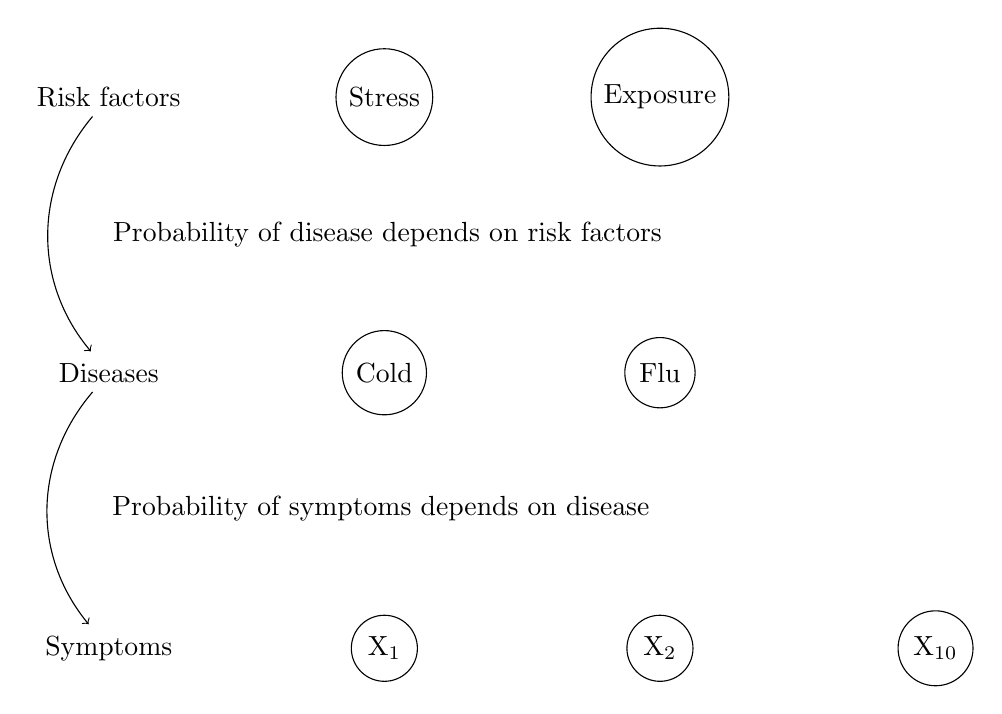
\begin{tikzpicture}[shorten >=1pt,node distance=3.5cm,on grid,auto,main node/.style={circle,draw}] 
    % \node[state, options?] (identifier) [placement] {display};
    \node[] (0) {Risk factors};
    \node[main node] (1) [right=of 0]{Stress};
    \node[main node] (2) [right=of 1] {Exposure};
    \node[] (3) [below=of 0] {Diseases};
    \node[main node] (4) [below=of 1] {Cold};
    \node[main node] (5) [right=of 4] {Flu};
    \node[] (6) [below=of 3] {Symptoms};
    \node[main node] (7) [right=of 6] {X$_{1}$};
    \node[main node] (8) [right=of 7] {X$_{2}$};
    \node[main node] (9) [right=of 8] {X$_{10}$};
    
    \path[->] 
    (0) edge [bend right=40] node {\qquad Probability of disease depends on risk factors} (3)
    (3) edge [bend right=40] node {\qquad Probability of symptoms depends on disease} (6);
    \end{tikzpicture}
    \\ \\
    Write psuedocode that calculates the probability of flu \textit{conditioned on observing} that the patient has had exposure to a sick friend and that they are experiencing symptom 2 (sore throat). In terms of random variables P(Flu = 1 | Exposure = 1 and X$_2$ = 1):
    \begin{quote}
        \texttt{def probFlu(): // P(Flu = 1 | Exposure = 1 and X2 = 1)}
    \end{quote}
    We know the prior probability for Stress is 0.5 and Exposure is 0.1.\\ \\
    You are given functions \texttt{probCold(s, e)} and \texttt{probFlu(s, e)} which return the probability that a patient has a cold or flu, given the state of the risk factors stress (\texttt{s}) and exposure (\texttt{e}).\\ \\
    You are given a function \texttt{probSymptom(i, f, c)} which returns the probability that the \texttt{i}th symptom ($X_i$) takes on value 1, given the state of cold (\texttt{c}) and flu (\texttt{f}): $P(X_i = 1|F = f,C = c)$.
    
    \begin{enumerate}
        \item Write psuedocode that calculates \texttt{probFlu()} using \textbf{Joint Sampling}.
        \item (Reach) Write pseudocode that calculates \texttt{probFlu()} without using sampling.
        \begin{quote}
            Note: Causality implies the following: (1) that risk factors are independent. (2) all diseases are independent of one another conditioned on risk factors. (3) that all symptoms are independent of one another conditioned on knowing the state of diseases:
            \small{
            \begin{equation}
                P(S = s, E = e) = P(S = s)P(E = e)
            \end{equation}
            \begin{equation}
                P(C = c, F = f |S = s, E = e) = P(C = c|S = s, E = e) \cdot P(F = f |S = s, E = e)
            \end{equation}
            \begin{equation}
                P(\text{symptoms}|F = f,C = c) = \prod_j P(X_j = k_j|F = f,C = c)
            \end{equation}
            }
        \end{quote}
        ``Reach'' means I don't expect CS109 students to be able to solve the problem. But thinking about it will be useful. Show your work. If you get stuck, explain what is hard.
    \end{enumerate}
    
    \begin{shaded}
    \begin{answer}
    
    \end{answer}
    \end{shaded}
    
}
\end{enumerate}


\end{document}